

% This is a simple sample document.  For more complicated documents take a look in the exercise tab. Note that everything that comes after a % symbol is treated as comment and ignored when the code is compiled.

\documentclass{article} % \documentclass{} is the first command in any LaTeX code.  It is used to define what kind of document you are creating such as an article or a book, and begins the document preamble

\usepackage{amsmath} % \usepackage is a command that allows you to add functionality to your LaTeX code
\usepackage{tikz}
\usetikzlibrary{automata, positioning}

\title{%
  CW 1.3, Automata. \\
  \large F29LP}
\author{%
Yoav Levi\\
\small H00347035
} % Sets authors name
\date{\today} % Sets date for date compiled

% The preamble ends with the command \begin{document}
\begin{document} % All begin commands must be paired with an end command somewhere
    \maketitle % creates title using information in preamble (title, author, date)
    
    \section{/$(ab)*$/} % creates a section
    \section{/$(b*a)+a+b[ab]*$/}
    \section{NFA}
    \begin{enumerate}
    \item
        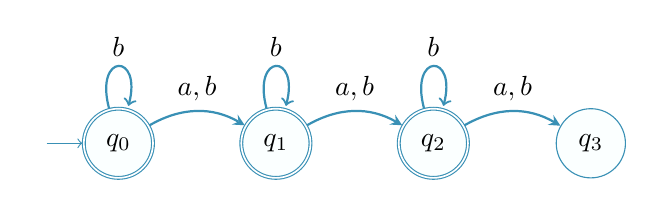
\begin{tikzpicture} [draw=cyan!70!black,
            node distance = 2cm, 
            on grid, 
            auto]
            \tikzstyle{every state}=[fill={rgb:cyan,0.3;white,20}]
         
            % State q0 
            \node (q0) [state, 
                initial, 
                accepting, 
                initial text = {}] {$q_0$};
            
            % State q1    
            \node (q1) [state,
                accepting, 
                right = of q0] {$q_1$};
            
            % State q2    
            \node (q2) [state,
                accepting,
                right = of q1] {$q_2$};
            
            % State q1    
            \node (q3) [state,
                right = of q2] {$q_3$};
            
            % Arrows
            \path [-stealth, thick]
                (q0) edge[bend left] node {$a,b$}   (q1)
                (q1) edge[bend left] node {$a,b$}   (q2)
                (q2) edge[bend left] node {$a,b$}   (q3)
            
                (q0) edge [loop above]  node {$b$}()
                (q1) edge [loop above]  node {$b$}()
                (q2) edge [loop above]  node {$b$}();
        \end{tikzpicture}
    \item 
    \end{enumerate}
    \section{/$a*(ba\{2,\})*$/}

\end{document} % This is the end of the document
